Before going deep into structural properties of decomposable digraphs we first need to establish what a graph is.
For some graph $G(V,E)$ where $V$ and $E$ are two sets contaning the vertices (also commonly called nodes) and egdes of the graph respectivlely.
%Example $V=\lbrace a,b,c \rbrace$ then $a,\ b$ and $c$ are three distinct vertices of the graph $G$ and the only vertices of $G$.
We define the \textbf{size} of the graph to be the number of vertices $|V|$ this is also known as \textbf{cardinality} of $V$.
%In the case of the example the size of $G$ $|V|=3$ it is also called the order of a graph.
An \textbf{edge} $e \in E$ where $e \equiv (a, b)$ and $\{ a, b \} \subseteq V$ then $e$ is an edge in $G$, $e$ is said to be \textbf{incedent} to $a$ and $b$. 
We call $a,b \in V$ \textbf{adjecent} if there is an edge $(a,b)$ or $(b,a)$ (an edge between the two given vertices is said to be adjecent).
If an edge goes from and to the same vertex $(a,a)$ it is called a \textbf{loop}.
The set of edges $e_1, \dots, e_k$ is usally describe whit the letter $E$ where each edge contains a pair of vertices that are adjecent. \\
In a graph we have something called a \textbf{walk} which is a alternately ordering of vertices an edges in the graph $G$ where the edge in between the two vertices in the ordering is an edge between the vertices in $G$ (for $a,e_1,b$ to be a walk the edge $e_1$ has to be between $a$ and $b$).
We call a walk closed if the first vertex in the walk is the same as the last.\\
A \textbf{path} in a graph is a walk where each vertex in the ordering can only apear one time. A cycle is a closed walk where the only vertex pressent more then one time is the first vertex(for the walk to be closed the first vertex has to apear last to also called a closed path).

%The describe example can be seen in figure \autoref{fig:graph}.
\begin{figure}[!h]
    \begin{subfigure}{0.48\textwidth}
        \centering
        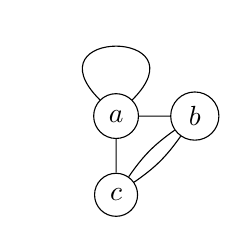
\begin{tikzpicture}
            [main/.style ={draw,circle}]
            \node[main] (a){$a$};
            \node[main] (b)[right of = a]{$b$};
            \node[main](c)[below of= a]{$c$};
            \draw (a) to (b) (c) to (a) (c) to [bend right =10](b) (c) to [bend left =10](b); 
            \draw (a) to [loop,red] (a);
        \end{tikzpicture} 
        \label{fig:graph}
        \caption{graph $G(V,E)$ is an example of a graphs, the red edge is a loop, and all pair of vertices in this graph is adjecent.}
    \end{subfigure}
   \begin{subfigure}{0.48\textwidth}
    \centering
        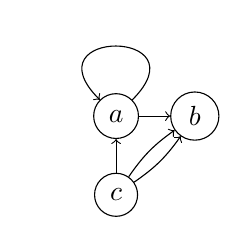
\begin{tikzpicture}
            [main/.style ={draw,circle}]
            \node[main] (a){$a$};
            \node[main] (b)[right of = a]{$b$};
            \node[main](c)[below of= a]{$c$};
            \draw[->] (a) to (b) ;
            \draw[->](c) to (a) ;
            \draw[->](c) to [bend right =10](b) ;
            \draw[->](c) to [bend left =10](b); 
            \draw[->] (a) to [loop,red] (a);
        \end{tikzpicture} 
        \label{fig:digraph}
        \caption{This is an oriantation of the edges in the graph which makes this a digraph}
   \end{subfigure}
\end{figure}


Before delving more specific into graphs and digraphs we must establish some important prerequisite and properties. 
A graph is called \textbf{simple} if there is no loops and no multiple edges. 
With multiple edges it means multiple edges between the same pair of vertices like in figure \autoref{fig:graph} between $b$ and $c$.
\begin{figure}[!h]
	\centering
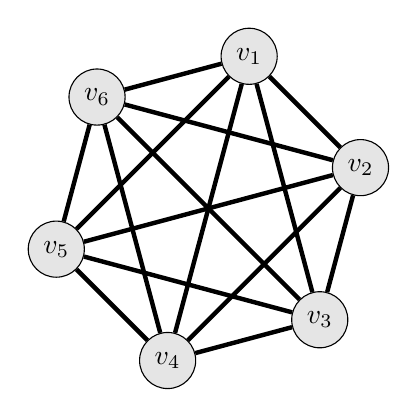
\begin{tikzpicture}[
	xs/.style = {xshift=#1 mm},
	ys/.style = {yshift=#1 mm}]
	
	\def \n {6}
	\def \radius {2cm}
	\def \margin {8} % margin in angles, depends on the radius
	
	\foreach \s in {1,...,\n}
	{
		\node[draw, circle][fill=gray!20!white] (\s) at ({360/\n * -(\s+3.75)}:\radius) {$v_\s$};
	}
    \draw[ultra thick] (1) -- (2) (1) -- (3) (1) -- (4) (1) -- (5) (1) -- (6);
    \draw[ultra thick] (2) -- (3) (2) -- (4) (2) -- (5) (2) -- (6);
    \draw[ultra thick] (3) -- (4) (3) -- (5) (3) -- (6);
    \draw[ultra thick] (4) -- (5) (4) -- (6);
    \draw[ultra thick] (5) -- (6);
\end{tikzpicture}
\caption{Complete graph with 6 vertices.}
\label{fig:complete}
\end{figure}

A graph is \textbf{connected} if there exists a path between all pair of vertices in the graph and \textbf{disconnected} otherwise.
A graph is called \textbf{complete} if there for all pair of vertices in the graph is an edge between them see \autoref{fig:complete}.\\

If we instead og an edges have \textbf{arcs} between the vertices we call it a \textbf{digraph}.
An arc is describe just like an egde with two adjecent vertices $(a,b)$ the first vertex mentioned in an arc is the vertex \textbf{from} where the arc starts, the second vertex is the one the arc is pointing \textbf{to}. The set of arcs is normaly denoted $A$ like the set of edges is denoted $E$
So the arc $(a,b)$ goes from $a$ to $b$, if you wanted it the other way around the arc is $(b,a)$.
These graph contaning only arcs and no edges is called a digraph $G(V,A)$ which is what we in this project are focusing on.\\

in a digraph a graph we have something called the underlying graph. 
An underlying graph of a digraph is where all arcs are replaced by edges (edge is used every time we talk about undirected edges between vertices, when direction is mentioned it is called an arc).
A digraph is connected if the underlying graph is connected, (also called weakly connected), a digraph can be strongly-connected and semi connected too.
A digraph is called semi connected if there for each pair $u$ and $v$ exists a path from either $u$ to $v$ or $v$ to $u$. 
It is said to be strongly connected if for each pair of vertices $u$ and $v$ there exists a path from both $u$ to $v$ and $v$ to $u$.

We can use these to describe som specific collection of graphs as the graph tournaments.
tournaments is a digraph where the underlying graph is complete. 
An underlying graph of a digraph is where all arcs are replaced by edges (edge is used every time we talk about undirected edges between vertices, when direction is mentioned it is called an arc).
So a complete graph of order 5 any orientation of the edges concludes in a tournament.
If instead of replacing the one edge by one arc in either direction, but instead replace it by two arcs the digraph is called semicomplete.

The reason for grouping the digraphs into smaller collections of digraphs (like tournaments is a smaller collection of semicomplete digraphs) is because of problems is easy describe on specific graphs than general graphs.

We have these graph called NP-hard problems which sometimes sound easy solvable for graphs but only for some specific graphs we know how to solve it in polynomial time. 
\begin{definition}
    define NP-hard problems
\end{definition}

In this paper we focusing on the specific digraphs that are decomposable. 
A decomposable digraph is a digraph $D=H[G_1,G_2,\dots,G_|H|]$ where each $G_i$ is disconnected graphs replacing each vertex of the digraph $H$. ...
